\chapter{Schémas aux différences compacts}

\section{Opérateux aux différences en dimension 1}

\subsection{Notations}
\label{sec:notation_1D}

On considère $\Omega = [a,b]$, $a<b$, un intervalle de $\mathbb{R}$ de longueur $L=b-a$. Nous utilisons les lettres latines pour noter les fonctions continues : $f(x)$, $u(x)$, ... $x \in \Omega$. Pour $u$ et $v$, des fonctions définies sur $\Omega$, le produit scalaire dans $L^2 ( \Omega )$ est défini par
\begin{equation}
(u,v) = \gint_{\Omega} u(x) \bar{v}(x) dx = \gint_{a}^b u(x) \bar{v}(x) dx.
\end{equation}
Pour $u$ et $v$ à valeurs réelles, on a
\begin{equation}
(u,v) = \gint_{a}^b u(x) v(x) dx.
\end{equation}
La norme sur $L^2(\Omega)$ est donnée par :
\begin{equation}
\| u \|_{L^2(\Omega)} = \sqrt{(u,u)}
\end{equation}
Pour $u \in L^{\infty}(\Omega)$, on note
\begin{equation}
\| u \|_{\infty} = \sup_{x\in\Omega} |u(x)|.
\end{equation}
Une fonction $u : x \in \mathbb{R} \mapsto u(x) \in \mathbb{R}$ est \textit{périodique} de période $L$ si 
\begin{equation}
u(x+L) = u(x) \text{, } \forall x \in \Omega.
\end{equation}
En particulier, on a $u(a)=u(b)$.

On considère une grille régulière sur $\Omega$ constituée de $N \geq 1$ points :
\begin{equation}
a=x_0 < x_1 < \ldots < x_{N-1} < x_N = b,
\end{equation}
où les valeurs $x_i$ sont définies par :
\begin{equation}
x_i = a + ih\text{, } i = 0,1, \ldots,N \text{ et } h = \dfrac{b-a}{N} \text{le pas d'espace}. 
\end{equation}

\begin{figure}[htbp]
\begin{center}
\begin{tikzpicture}[scale=1.8]
	\draw [>=stealth, <->] (-2,0.2) -- (-1,.2) ;
	\draw (-1.5,.3) node[above] {$h$} ;
	\draw (-3,0) -- (3,0) ;
	\draw (-3,0) node {$\times$} ;
	\draw (-3,-.2) node[below] {$x_0=a$} ;
	\draw (-2,0) node {$\bullet$} ;
	\draw (-2,-.2) node[below] {$x_1$} ;
	\draw (-1,0) node {$\bullet$} ;
	\draw (-1,-.2) node[below] {$x_2$} ;
	\draw (0,-.2) node[below] {$\ldots$} ;
	\draw (1,0) node {$\bullet$} ;
	\draw (1,-.2) node[below] {$x_{N-2}$} ;
	\draw (2,0) node {$\bullet$} ;
	\draw (2,-.2) node[below] {$x_{N-1}$} ;
	\draw (3,0) node {$\times$} ;
	\draw (3,-.2) node[below] {$x_N =b$} ;
\end{tikzpicture}
\end{center}
\caption{Grille en dimension 1. Les symboles $\times$ désignent les points de bords, les symboles $\bullet$ désignent les points intérieurs de la grille.}
\label{fig:maillage1D}
\end{figure}

Les points $x_0=a$ et $x_N = a + L = b$ sont les points de bord du domaine et les points $(x_i)_{1 \leq i \leq N-1}$ désignent les points intérieurs. 

Nous distinguons trois types de données aux points de grille $x_i$, $0 \leq i \leq N$ :
\begin{enumerate}
\item Une \textit{fonction de grille} est une fonction définie uniquement aux points $(x_i)_{0 \leq i \leq N}$. Les fonctions de grilles sont notées en fonte gothique : $\mathfrak{u}$, $\mathfrak{v}$, ... 
On note
\begin{equation}
\mathfrak{u} = (\mathfrak{u}(x_0), \mathfrak{u}(x_1), \mathfrak{u}(x_2), ... , \mathfrak{u}(x_N)).
\end{equation}
De plus, $l^2_h$ désigne l'espace des fonctions de grille, $h>0$ fixé.
On munit cet espace du produit scalaire et de la norme associée :
\begin{equation}
(\mathfrak{u},\mathfrak{v})_h = h \gsum_{i=0}^N \mathfrak{u}(x_i) \mathfrak{v}(x_i) \text{,  } |\mathfrak{u}|_h^2 = h \gsum_{i=0}^N \mathfrak{u}(x_i)^2.
\end{equation}
On définit aussi la norme infinie pour les fonctions de grille :
\begin{equation}
\| \mathfrak{u} \|_{\infty} = \max_{0\leq i \leq N} |\mathfrak{u}(x_i)|.
\end{equation}
On notera abusivement 
\begin{equation}
\mathfrak{u}_j = \mathfrak{u}(x_j) \text{ pour tout } 0\leq j \leq N.  
\end{equation}

On note $l^2_{h,per}$ l'espace des fonctions de grilles périodiques si $\mathfrak{u} \in l^2_{h,per}$ alors $\mathfrak{u}(x_0) = \mathfrak{u}(x_N)$. Le produit scalaire et la norme associée dans $l^2_{h,per}$ sont
\begin{equation}
(\mathfrak{u},\mathfrak{v})_{h,per} = h \gsum_{i=1}^N \mathfrak{u}(x_i) \mathfrak{v}(x_i) \text{,  } |\mathfrak{u}|_h^2 = h \gsum_{i=1}^N \mathfrak{u}(x_i)^2 \text{ avec} \mathfrak{u}, \mathfrak{v} \in l^2_{h,per}.
\end{equation}
La norme infinie dans $l^2_{h,per}$ est
\begin{equation}
\| \mathfrak{u} \|_{\infty} = \max_{1\leq i \leq N} |\mathfrak{u}(x_i)|.
\end{equation}

\item Les lettres latines capitales désignent les vecteurs de $\mathbb{R}^{N+1}$ et les matrices de $\mathbb{M}_{N+1}(\mathbb{R})$. Par exemple, soit le vecteur $U \in \mathbb{R}^{N+1}$ des composantes de $\mathfrak{u} \in l^2_h$ :
\begin{equation}
U = \begin{bmatrix}
\mathfrak{u}_0 \\ \mathfrak{u}_1 \\ \vdots \\ \mathfrak{u}_N
\end{bmatrix} =
\begin{bmatrix}
\mathfrak{u}(x_0) \\ \mathfrak{u}(x_1) \\ \vdots \\ \mathfrak{u}(x_N)
\end{bmatrix}
\end{equation}
La norme euclidienne sur $\mathbb{R}^{N+1}$ est notée $|U|$. Elle induit une norme pour les matrices $A \in \mathbb{M}_{N+1}(\mathbb{R})$ définie par
\begin{equation}
|A|_2 = \sup_{U \neq 0} \dfrac{|AU|}{|U|}.
\end{equation}
Si $A$ est symétrique alors :
\begin{equation}
|A|_2 = \rho(A) := \max \left\lbrace |\lambda| \text{ tels que } \lambda \in \Sp (A) \right\rbrace.
\end{equation}
$\rho(A)$ est nommé \textit{rayon spectrale} de $A$.
La norme infinie de $U$ est donnée par :
\begin{equation}
|U|_{\infty} = \max_{1 \leq i \leq N+1} |U_i|.
\end{equation}
La norme sur $\mathbb{M}_{N+1}(\mathbb{R})$ subordonnée à $|\cdot|_{\infty}$ est
\begin{equation}
|A|_{\infty} = \sup_{U \neq 0} \dfrac{|AU|_{\infty}}{|U|_{\infty}} = \max_{1 \leq i \leq N+1} \gsum_{j=1}^{N+1} |A_{i,j}|.
\end{equation}

\item Soit $u: x \in \Omega \mapsto u(x)$, on définit la \textit{fonction de grille} $u^*$ associée à $u$ par :
\begin{equation}
u^*_i = u^*(x_i) \text{ pour } 0 \leq i \leq N.
\end{equation}
$u^*$ est donc la restriction de $u$ aux points de la grille. Si $u$ est une fonction périodique, alors 
\begin{equation}
u^*_i = u^*(x_i) \text{ pour } 1 \leq i \leq N.
\end{equation}
\end{enumerate}

Nous distinguons $l^2_h$, l'espace des fonctions de grilles, de $\mathbb{R}^{N+1}$ même si ces deux espaces sont isomorphes.

Cette distinction permet de faire une claire différences entre :
\begin{itemize}
\item les opérateurs aux différences finies, qui agissent sur les fonctions de grilles,
\item les matrices, qui agissent sur les vecteurs.
\end{itemize}
Les fonctions de grilles contiennent toutes les échelles nécessaires dans le contexte physique alors que les vecteurs sont sans dimension. De plus, le raisonnement au niveau discret est plus naturel avec les fonctions de grilles. Il s'effectue d'une façon abstraite à l'aide d'opérateurs aux différences. En revanche, le codage est effectuée dans le cadre de l'algèbre linéaire.

Par exemple, si $u : x \in \Omega \mapsto u(x) \in \mathbb{R}$ régulière telle que $u(a) = u(b) = 0$ alors $(\partial_x u)^*$ désigne la fonction de grille associée à la dérivée première de $u$. On peut approcher cette donnée à l'aide de la fonction de grille $\mathfrak{u}_x$ obtenue grâce à l'opérateur $\delta_x$ agissant sur les fonctions de grilles et donné par
\begin{equation}
\mathfrak{u}_{x,j} = \delta_x u^*(x_j) = \dfrac{u(x_{j+1}) - u(x_{j-1})}{2h}.
\end{equation}
En effet, par développement de Taylor, on a 
\begin{equation}
u(x_j+h) = u(x_j) + h \partial_x u(x_j) + \dfrac{h^2}{2} \partial_x^2 u(x_j) + \dfrac{h^3}{6} \partial_x^3 u(\xi) \text{ avec } \xi \in [x_j, x_j+h].
\end{equation}
De la même manière, en $x_j-h$, on a 
\begin{equation}
u(x_j-h) = u(x_j) - h \partial_x u(x_j) + \dfrac{h^2}{2} \partial_x^2 u(x_j) - \dfrac{h^3}{6} \partial_x^3 u(\eta) \text{ avec } \eta \in [x_j-h, x_j].
\end{equation}
On a alors
\begin{align*}
\delta_x u^*(x_j) & = \dfrac{u(x_{j+1}) - u(x_{j-1})}{2h}\\
                  & = \dfrac{1}{2h} \left[ 2h \partial_x u(x_j) + \dfrac{h^3}{6} \partial_x^3 u(\xi) + \dfrac{h^3}{6} \partial_x^3 u(\eta) \right]\\
                  & = \partial_x u(x_j) + \dfrac{h^2}{2} \left[ \dfrac{1}{6} \partial_x^3 u(\xi) + \dfrac{1}{6} \partial_x^3 u(\eta) \right] \\
                  & = \partial_x u(x_j) + \dfrac{h^2}{6} \partial_x^3 u(\gamma) \text{ avec } \gamma \in ]x_j-h , x_j+h[ \text{ par théorème des valeurs intermédiaires.}
\end{align*}
Ainsi l'erreur de troncature est une fonction de grille définie en chaque point du $x_j$ par
\begin{align*}
\mathfrak{t}(x_j) & = \delta_x u^*(x_j) - \delta_x u^*(x_j)\\
                  & = \dfrac{h^2}{6} \partial_x^3 u(\gamma) \text{ avec } \gamma \in ]x_j-h , x_j+h[.
\end{align*}










\subsection{Opérateurs de translations}

On considère $\Omega = [0,L]$. Les notations employées sont celles de la partie \ref{sec:notation_1D} dans le contexte périodique.

\begin{definition}
L'\textit{opérateur de translation} $\tau_p$, $p \in \mathbb{Z}$, est tel que si $\mathfrak{u}$ est une fonction de grille périodique alors pour tout $1 \leq i \leq N$
\begin{equation}
(\tau_p \mathfrak{u})_i = \mathfrak{u}_{i+p}.
\end{equation}
\end{definition}

Cet opérateur permettra de définir les opérateurs aux différences. L'opérateur $\tau_p$ agit sur les fonctions de grille périodiques $u^*$ par :
\begin{equation}
(\tau_p u^*)_i = u^*_{i+p} = u(x_{i+p}).
\end{equation}
en considérant les propriétés de périodicité lorsque $i+p > N$ ou $i+p<1$.
De la même manière, on définit l'opérateur $\tau$ par 
\begin{equation}
\tau = \tau_{1}
\end{equation}
On note $\tau^p$, où $p$ est un entier naturel, l'opérateur
\begin{equation}
\begin{array}{rcl}
\tau^0 & = & id\\
\tau^p & = & \underbrace{\tau \circ \tau \circ \tau \circ \cdots \circ \tau}_{p \text{ fois.}}
\end{array}
\end{equation}

\begin{proposition}
L'égalité suivante est vérifiée :
\begin{equation}
\tau^p = \tau_p
\end{equation}
En particulier, on a $\tau^N = \tau_N = id$.
\end{proposition}

\begin{proof}
Résultat vrai par récurrence immédiate.
\end{proof}
Il est intéressant de rechercher les valeurs propres et les vecteurs propres de $\tau$ de manière à en déduire le spectre des opérateurs qui sont issus de $\tau$.


\begin{proposition}
Les fonctions propres de $\tau$ sont les fonctions de grilles $\mathfrak{u}^k$ vérifiant :
\begin{equation}
\mathfrak{u}_j^k = \exp \left[ i j \dfrac{2 \pi k}{N} \right]
\label{eq:vecteurpropre_tau}
\end{equation}
Chaque vecteur propre est associé à la valeur propre $\lambda^k$ avec 
\begin{equation}
\lambda = \exp \left[ i \dfrac{2 \pi}{N} \right].
\end{equation}
et $1 \leq k \leq N$.
\end{proposition}


\begin{proof}
On calcule $(\tau \mathfrak{u}^k)_j$ :
\begin{equation}
(\tau \mathfrak{u}^k)_j = \exp \left[ i (j+1) \dfrac{2 \pi k}{N} \right] = \exp \left[ i j \dfrac{2 \pi k}{N} \right] \exp \left[ i \dfrac{2 \pi k}{N} \right]  = \mathfrak{u}_j^k \lambda^k
\end{equation}
De plus, il est facile de voir que $\mathfrak{u}$ vérifie l'hypothèse de périodicité, d'où le résultat.
\end{proof}
Si $P(X)$ est un polynôme en $X$ de degré au plus $N-1$, \textit{i.e.} $P \in \mathbb{R}_{N-1} [x]$ alors les valeurs propres et fonctions propres de $P(\tau)$ sont connues.

\begin{proposition}
Les fonctions propres de $P(\tau)$ sont les fonctions de grilles $\mathfrak{u}^k$ vérifiant :
\begin{equation}
\mathfrak{u}_j^k = \exp \left[ i j \dfrac{2 \pi k}{N} \right]
\end{equation}
Chaque vecteur propre est associé à la valeur propre $P(\lambda^k)$ avec 
\begin{equation}
\lambda = \exp \left[ i \dfrac{2 \pi}{N} \right]
\end{equation}
avec $1 \leq k \leq N$.
\label{prop:eigen_tau}
\end{proposition}

\begin{proof}
Soient $(a_i)_{0 \leq i \leq N-1}$ des réels tels que 
\begin{equation}
P(x) = \gsum_{i=0}^{N-1} a_i x^i,
\end{equation}

Calculons $P(\tau) \mathfrak{u}^k$. Soit $j$ un entier compris entre $1$ et $N$, 

\begin{equation}
(P(\tau) \mathfrak{u}^k)_j = \left( \gsum_{i=1}^{N} a_i \tau_ p \mathfrak{u}^k \right)_j = \gsum_{i=1}^{N} a_i (\lambda^k)^p \mathfrak{u}^k_j = P(\lambda^k) \mathfrak{u}^k_j
\end{equation}

d'où le résultat.
\end{proof}
L'opérateur de translation $\tau$ agit sur les fonctions de grilles $\mathfrak{u}$. Il est associé à $T \in \mathcal{M}_N \left( \mathbb{R} \right)$ la matrice agissant sur les vecteurs $U$ de $\mathbb{R}^N$
\begin{equation}
U = \begin{bmatrix}
\mathfrak{u}_1\\
\mathfrak{u}_2\\
\vdots\\
\mathfrak{u}_{N}\\
\end{bmatrix}
\end{equation}
La matrice $T$ est donnée par

\begin{equation}
T = \begin{bmatrix}
0 & 1 &   &   &   \\ 
  & 0 & 1 & (0) &   \\ 
  &   & \ddots & \ddots &   \\ 
  & (0) &   & 0 & 1 \\ 
1 &   &   &   & 0
\end{bmatrix} 
\end{equation}

La matrice $T$ agit sur un vecteur $U = \begin{bmatrix}
U_1 & U_2 & \cdots & U_{N} 
\end{bmatrix}^T \in \mathbb{R}^N $ de telle manière que, pour tout $1 \leq j \leq N$, on a 

\begin{equation}
(TU)_j = U_{j+1}
\end{equation}
Les propriétés concernant les valeurs propres de $\tau$ sont aussi vérifiées par $T$.

\begin{proposition}
\begin{itemize}
\item Les valeurs propres de $T$ sont les valeurs $(\lambda^k)_{1 \leq k \leq N}$ avec 
\begin{equation}
\lambda = \exp \left[ i \dfrac{2 \pi}{N} \right].
\label{eq:eigenvalueT}
\end{equation}
les vecteurs propres associés sont donnés par $\left( U^k \right)_{1 \leq k \leq N}$ vérifiant :
\begin{equation}
U^k = \dfrac{1}{\sqrt{N}} \begin{bmatrix}
\mathfrak{u}_0^k\\
\mathfrak{u}_1^k\\
\vdots \\
\mathfrak{u}_{N-1}^k
\end{bmatrix}
\label{eq:eigenvectorT}
\end{equation}
où $\mathfrak{u}^k$ est la fonction de grille \eqref{eq:vecteurpropre_tau}.

\item Si $P \in \mathbb{R}_{N-1}[X]$ alors les valeurs propres de $P(T)$ sont 
\begin{equation}
P(\lambda)
\end{equation}
avec $\lambda$ donné par \eqref{eq:eigenvalueT}.
\end{itemize}
Les vecteurs propres sont donnés par \eqref{eq:eigenvectorT}.
\label{prop:eigen_P(tau)}
\end{proposition}

Les vecteurs propres de $T$ donnés par \eqref{eq:eigenvectorT} forment clairement une base orthonormée pour le produit scalaire usuel, en effet on a 
\begin{equation}
(\bar{U^k})^T \cdot U^{k'} = \delta_{k,k'}
\end{equation}
où $\delta_{k,k'}$ désigne le symbole de Kronecker et vaut $1$ si $k=k'$ et $0$ sinon.













\subsection{Opérateur centré d'ordre 2}

Introduisons l'\textit{opérateurs aux différences centré} usuel
\begin{equation}
\delta_x = \dfrac{\tau_1 - \tau_{-1}}{2h}
\end{equation}
Appliqué à la fonction de grille $\mathfrak{u}$, cet opérateur vérifie 
\begin{equation}
\delta_x \mathfrak{u}_i = \dfrac{\mathfrak{u}_{i+1} - \mathfrak{u}_{i-1}}{2h} \text{ pour } 1 \leq i \leq N.
\end{equation}
Il s'agit d'un opérateur permettant d'approcher la dérivée première au sens où

\begin{proposition}
Soit $u: x \in \Omega \mapsto u(x) \in \mathbb{R}$ et $u^*$ la fonction de grille correspondante. Si $u \in \mathcal{C}^3 (\Omega)$ alors 
\begin{equation}
\delta_x u^*_i - u'(x_i) = \dfrac{h^2}{12} \left[ u^{(3)}(\xi_i) + u^{(3)}(\eta_i) \right]  \text{ avec } \xi_i , \eta_i \in [x_{i-1}, x_{i+1}],
\end{equation}
\end{proposition}

\begin{proof}
Comme $u$ est de classe $\mathcal{C}^3$, on considère les développements de Taylor :
\begin{equation}
u(x_i+h) = u(x_i) + h u'(x_i) + \dfrac{h^2}{2} u''(x_i) + \dfrac{h^3}{6} u^{(3)} (\eta_i) \text{ avec } \eta_i \in [x_i, x_{i+1}]
\end{equation}
et celui en $x-h$ :
\begin{equation}
u(x_i-h) = u(x_i) - h u'(x_i) + \dfrac{h^2}{2} u''(x_i) - \dfrac{h^3}{6}u^{(3)}(\xi_i) \text{ avec } \xi_i \in [x_{i-1}, x_{i}]
\end{equation}
Alors par différence, on retrouve la formule souhaitée : 
\begin{equation}
\delta_x u^*_i = u'(x_i) + \dfrac{h^2}{12} \left[ u^{(3)}(\xi_i) + u^{(3)}(\eta_i) \right]  \text{ avec } \xi_i, \eta_i \in [x_{i-1}, x_{i+1}],
\end{equation}
\end{proof}

Ainsi, $\delta_x$ est un opérateur d'approximation de la dérivée première à l'ordre 2. L'opérateur $\delta_x$ est associé à une matrice $K$ de telle manière que si 
\begin{equation}
U = \begin{bmatrix}
\mathfrak{u}_1\\
\mathfrak{u}_2\\
\vdots\\
\mathfrak{u}_{N}\\
\end{bmatrix} \in \mathbb{R}^N \text{ et } U_x = \begin{bmatrix}
\delta_x \mathfrak{u}_1\\
\delta_x \mathfrak{u}_2\\
\vdots\\
\delta_x \mathfrak{u}_{N}\\
\end{bmatrix} \in \mathbb{R}^N
\end{equation}
alors
\begin{equation}
U_x = K U
\end{equation}
avec la matrice $K$ donnée par
\begin{equation}
K = \dfrac{1}{2h} \begin{bmatrix}
0    & 1    &    &    &     & -1 \\
-1   & 0    & 1  &    & (0) &    \\
     & -1   & 0  & 1  &     &    \\
     &      & \ddots  & \ddots  & \ddots    &    \\
     & (0)  &    & -1 & 0   & 1  \\
1    &      &    &    & -1  & 0  \\
\end{bmatrix}
\end{equation}
La matrice $K$ est antisymétrique. En particulier, on remarque que 
\begin{equation}
K = \dfrac{1}{2h} \left( T - T^{N-1} \right)
\end{equation}
donc d'après la proposition \ref{prop:eigen_P(tau)}, les valeurs propres de $K$ sont 
\begin{equation}
\theta^k = \dfrac{1}{2h} \left[ \exp \left( \dfrac{2 i \pi k}{N} \right) - \exp \left( \dfrac{-2 i \pi k}{N} \right) \right] = \dfrac{i}{h} \sin \left( \dfrac{2 \pi k}{N} \right) \text{ avec } 1 \leq k \leq N.
\end{equation}
En particulier, on remarque que $\theta^N = 0$ donc la matrice $K$ n'est pas inversible.












\subsection{Schémas Hermitien}

Dans son article \cite{Lele1991}, S. K. Lele présente une méthode permettant d'approcher la dérivée en un point en ajoutant une partie implicite aux schémas classiques. Définissons l'opérateur de Simpson $\sigma_{x}$ par :

\begin{equation}
\sigma_{x}  = \dfrac{1}{6} \tau_1 + \dfrac{4}{6} id + \dfrac{1}{6}\tau_{-1}
\end{equation}
En particulier, si $\mathfrak{u}$ est une fonction de grille périodique,
\begin{equation}
\sigma_x \mathfrak{u}_j = \dfrac{1}{6} \mathfrak{u}_{j+1} + \dfrac{4}{6} \mathfrak{u}_j + \dfrac{1}{6} \mathfrak{u}_{j-1}
\end{equation}

Les valeurs propres de $\sigma_x$ sont connues.
\begin{proposition}
Les valeurs propres de $\sigma_x$ sont 
\begin{equation}
\mu^k = \dfrac{2}{3} + \dfrac{1}{3} \cos \left( \dfrac{2 \pi k}{N} \right)
\end{equation}
avec $1 \leq k \leq N$. Chaque valeur propre est associé à la fonction propre $\mathfrak{u}^k$ avec 
\begin{equation}
\mathfrak{u}_j^k = \exp \left[ i j \dfrac{2 \pi k}{N} \right]
\end{equation}
\label{prop:vp_sigma}
\end{proposition}

\begin{proof}
La proposition \ref{prop:eigen_P(tau)} permet de voir que $\mathfrak{u}^k$ est la fonction propre associée à $\mu^k$ avec 
\begin{equation}
\mu^k = \dfrac{4}{6} + \dfrac{1}{6} \left( \exp \left[ i \dfrac{2 \pi k}{N} \right] + \exp \left[ - i \dfrac{2 \pi k}{N} \right] \right) = \dfrac{2}{3} + \dfrac{1}{3} \cos \left( \dfrac{2 \pi k}{N} \right).
\end{equation}
On a alors $N$ valeurs propres distinctes, d'où le résultat.
\end{proof}
En particulier, on remarque que 
\begin{equation}
\mu^k \neq 0 \text{ pour tout } 1 \leq k \leq N
\end{equation}
donc $\sigma_x$ est inversible.

\begin{corollaire}
L'opérateur $\sigma_x$ est inversible.
\end{corollaire}
De plus, on note que si $u : x \in \Omega \mapsto u(x) \in \mathbb{R}$ est une fonction suffisamment régulière, le résultat suivant est vérifié.

\begin{proposition}
Soit $u : x \in \Omega \mapsto u(x) \in \mathbb{R}$ une fonction de $\mathcal{C}^5 ( \Omega )$, soit $u^*$ la fonction de grille associée. On note $u'$ la dérivée de $u$ et $u'^*$ la fonction de grille associée. Alors 
\begin{equation}
\sigma_x u'^*_i - \delta_x u^*_i = \dfrac{h^4}{144} \left( u^{(5)}(\xi'_i) + u^{(5)}(\eta'_i) \right) - \dfrac{h^4}{240} \left( u^{(5)}(\xi_i) + u^{(5)}(\eta_i) \right)
\end{equation}
avec $\xi_i$, $\xi'_i$ dans $[x_i, x_{i+1}]$ et $\eta_i$, $\eta'_i$ dans $[x_{i-1}, x_{i}]$.
\label{prop:consistence_herm}
\end{proposition}

\begin{proof}
Comme $u$ est de classe $\mathcal{C}^5$, on considère les développements de Taylor-Lagrange :
\begin{equation}
u(x_i+h) = u(x_i) + h u'(x_i) + \dfrac{h^2}{2} u''(x_i) + \dfrac{h^3}{6}u^{(3)}(x_i) + \dfrac{h^4}{24}u^{(4)}(x_i) + \dfrac{h^5}{120}u^{(5)}(\eta_i) \text{ avec } \eta_i \in [x_i, x_{i+1}]
\end{equation}
et celui en $x_i-h$ :
\begin{equation}
u(x_i+h) = u(x_i) - h u'(x_i) + \dfrac{h^2}{2} u''(x_i) - \dfrac{h^3}{6}u^{(3)}(x_i) + \dfrac{h^4}{24}u^{(4)}(x_i) - \dfrac{h^5}{120}u^{(5)}(\xi_i) \text{ avec } \xi_i \in [x_{i-1}, x_{i}]
\end{equation}
Alors par différence, on retrouve la formule souhaitée : 
\begin{equation}
\delta_x u^*_i = u'(x_i) + \dfrac{h^2}{6} u^{(3)}(x_i) +  \dfrac{h^4}{240} \left( u^{(5)}(\xi_i) + u^{(5)}(\eta_i) \right),
\end{equation}

De la même manière, on a 
\begin{equation}
\sigma_x u'^*_i = u'(x_i) +  \dfrac{h^2}{6} u^{(3)}u(x_i) + \dfrac{h^4}{144} \left( u^{(5)}(\xi'_i) + u^{(5)}(\eta'_i) \right).
\end{equation}
Ainsi, on retrouve le résultat souhaité.
\end{proof}

L'opérateur $\sigma_x$ est inversible, donc on peut définir l'\textit{opérateur hermitien d'ordre 4} :
\begin{equation}
\delta_x^H = \sigma_x^{-1} \circ \delta_x
\label{def:herm_4}
\end{equation}
Il s'agit d'un opérateur d'approximation de la dérivée première, en effet

\begin{theoreme}
Soit $u : x \in \Omega \mapsto u(x) \in \mathbb{R}$ une fonction de $\mathcal{C}^5 ( \Omega )$, soit $u^*$ la fonction de grille associée, alors
\begin{equation}
| u'^* -  \delta_x^H u^* |_{\infty} \leq C h^4
\end{equation}
\label{prop:consistence_herm2}
\end{theoreme}

\begin{proof}
On a directement 
\begin{equation*}
\begin{array}{rcl}
| u'^* -  \delta_x^H u^* |_{\infty} & = & | \sigma_x^{-1} \left( \sigma_x u'^* - \delta_x u^* \right) |_{\infty} \\
	& \leq & \| \sigma^{-1}_x \|_{\infty} |\sigma_x u'^* - \delta_x u^* |_{\infty}\\
	& \leq & C h^4 \text{ d'après la proposition \ref{prop:consistence_herm},}
\end{array}
\end{equation*}
avec
\begin{equation}
C = \dfrac{1}{45} \| \sigma^{-1}_x \|_{\infty} \| u^{(5)} \|_{\infty}.
\end{equation}
\end{proof}

\begin{proposition}
Les valeurs propres de $\delta_x^H$ sont données par 
\begin{equation}
\omega^k = \dfrac{i}{h} \dfrac{\sin \left( \dfrac{2 \pi k}{N} \right)}{\dfrac{2}{3} + \dfrac{1}{3} \cos \left( \dfrac{2 \pi k}{N} \right)}
\end{equation}
avec $1 \leq k \leq N$. Chaque valeur propre est associé à la fonction propre $\mathfrak{u}^k$ avec 
\begin{equation}
\mathfrak{u}_j^k = \exp \left[ i j \dfrac{2 \pi k}{N} \right]
\end{equation}
\label{prop:vp_herm}
\end{proposition}

\begin{proof}
On a déjà vu dans la proposition \ref{prop:vp_sigma} que 
\begin{equation}
\sigma_x \mathfrak{u}^k = \varepsilon^k \mathfrak{u}^k.
\end{equation}
De plus, $\sigma_x$ est inversible, donc 
\begin{equation}
\sigma_x^{-1} \mathfrak{u}^k = \dfrac{1}{\varepsilon^k} \mathfrak{u}^k.
\end{equation}

On sait aussi que 
\begin{equation}
\delta_x \mathfrak{u}^k = \dfrac{i}{h} \sin \left( \dfrac{2 \pi k}{N} \right) \mathfrak{u}^k
\end{equation}
donc en composant par $\sigma_x^{-1}$, on obtient directement 
\begin{equation}
\delta^H_x \mathfrak{u}^k = \sigma_x^{-1} \delta_x \mathfrak{u}^k = \dfrac{i}{h} \dfrac{\sin \left( \dfrac{2 \pi k}{N} \right)}{\mu^k} \mathfrak{u}^k = \omega^k \mathfrak{u}^k.
\end{equation}
C'est à dire le résultat souhaité.
\end{proof}

On note $P$ l'opérateur associé à $\sigma_x$ agissant sur les vecteurs $U = [U_1, U_2, \ldots, U_N]^T \in \mathbb{R}^N$. $P$ s'exprime sous la forme suivante :
\begin{equation}
P = \dfrac{1}{6} 
\begin{bmatrix}
4 & 1 &   &   & 1 \\ 
1 & 4 & 1 & (0) &   \\ 
  & \ddots & \ddots & \ddots &   \\ 
  & (0) & 1 & 4 & 1 \\ 
1 &   &  & 1 & 4
\end{bmatrix}.
\end{equation}

Alors si
\begin{equation}
U = \begin{bmatrix}
\mathfrak{u}_1 \\
\mathfrak{u}_2 \\
\vdots \\
\mathfrak{u}_N \\
\end{bmatrix} \text{ et } 
U' = \begin{bmatrix}
\delta_x^H \mathfrak{u}_1 \\
\delta_x^H \mathfrak{u}_2 \\
\vdots \\
\delta_x^H \mathfrak{u}_N \\
\end{bmatrix}
\end{equation}
sont deux vecteurs de $\mathbb{R}^N$, la relation suivante est vérifiée :
\begin{equation}
P U' = K U.
\end{equation}

\begin{proposition}
La dérivée hermitienne $\delta_x^H$ est associée à la matrice $P^{-1}K$ dont les valeurs propres sont
\begin{equation}
\omega^k = \dfrac{i}{h} \dfrac{\sin \left( \dfrac{2 \pi k}{N} \right)}{\dfrac{2}{3} + \dfrac{1}{3}\cos \left( \dfrac{2 \pi k}{N} \right)}
\end{equation}
avec $1 \leq k \leq N$. Chaque valeur propre $\omega^k$ est associée à un vecteur propre $U^k$ donné par
\begin{equation}
U^k = \dfrac{1}{\sqrt{N}} \begin{bmatrix}
\mathfrak{u}^k_1 \\
\mathfrak{u}^k_2 \\
\vdots \\
\mathfrak{u}^k_N \\
\end{bmatrix}
\end{equation}
où $\mathfrak{u}^k_j$ est donné par \eqref{eq:vecteurpropre_tau}.
\label{prop:eigen_mat_hermitien}
\end{proposition}

Ainsi, dans la pratique, la dérivée hermitienne $\delta_x^H \mathfrak{u}$ en chaque point est calculée comme la solution d'un système linéaire. Cette solution peut être calculée grâce à la formule de Shermann-Morisson-Woodbury couplé à un solveur tridiagonal comme l'algorithme de Thomas.

\begin{proposition}
\textbf{(Formule de Shermann-Morisson-Woodbury)} Soient $A, B \in \mathcal{M}_N \left(\mathbb{R} \right)$ deux matrices inversibles telles que 
\begin{equation}
A = B + R S^T,
\end{equation}
avec $R$ et $S$ deux matrices de $\mathcal{M}_{N,n} \left(\mathbb{R} \right)$ avec $n \leq N$.
Alors l'inverse de $A$ peut s'écrire
\begin{equation}
A^{-1} = B^{-1} - B^{-1} R \left( Id + S^T B^{-1} R  \right)^{-1} S^T B^{-1}.
\label{eq:SMW}
\end{equation}
\end{proposition}

\begin{proof}
Il suffit de vérifier que 
\begin{equation}
\left( B + R S^T \right) \left( B^{-1} - B^{-1} R \left( Id + S^T B^{-1} R  \right)^{-1} S^T B^{-1} \right) = Id.
\end{equation}
\end{proof}

Dans le cas où $n \lll N$, $A$ est une petite perturbation de la matrice $B$ de la forme 
\begin{equation}
A = B + \delta B
\end{equation}
avec $\rang  (\delta B) $ "petit". Si on peut facilement calculer l'inverse de $B$ la formule de Shermann-Morisson-Woodbury \eqref{eq:SMW} donne un algorithme efficace de résolution du système
\begin{equation}
A X = b.
\end{equation} 

\begin{center}
\begin{minipage}[H]{12cm}
  \begin{algorithm}[H]
    \caption{: Algorithme de Shermann-Morisson-Woodbury}\label{alg:SMW}
    \begin{algorithmic}[1]
	\State Calcul de $V_1 = B^{-1} b$,
	\State Calcul de $V_2 = S^T V_1$,
	\State Calcul de $V_3 = (Id + S^T B^{-1}R)^{-1} V_2$ (résolution d'un système de petite taille),
	\State Calcul de $V_4 = R V_3$,
	\State Calcul de $V_5 = B^{-1} V_4$,
	\State Calcul de $X = V_1 - V_5$.
    \end{algorithmic}
    \end{algorithm}
\end{minipage}
\end{center}

\begin{proposition}
Soit $P$ et $\tilde{P}$ les matrice donnée par 
\begin{equation}
P = \dfrac{1}{6} 
\begin{bmatrix}
4 & 1 &   &   & 1 \\ 
1 & 4 & 1 & (0) &   \\ 
  & \ddots & \ddots & \ddots &   \\ 
  & (0) & 1 & 4 & 1 \\ 
1 &   &  & 1 & 4
\end{bmatrix} \text{ et }
\tilde{P} = \dfrac{1}{6} 
\begin{bmatrix}
4 & 1 &   &   &  \\ 
1 & 4 & 1 & (0) &   \\ 
  & \ddots & \ddots & \ddots &   \\ 
  & (0) & 1 & 4 & 1 \\ 
 &   &  & 1 & 4
\end{bmatrix}.
\end{equation}
Alors 
\begin{equation}
P = \tilde{P} + R S^T
\end{equation} 
avec 
\begin{equation}
R = \dfrac{1}{6}\begin{bmatrix}
1 & 0 \\ 
0 & \vdots \\ 
\vdots & \vdots \\ 
\vdots & 0 \\ 
0 & 1
\end{bmatrix} \text{ et } 
S = \begin{bmatrix}
0 & 1 \\ 
\vdots & 0 \\ 
\vdots & \vdots \\ 
0 & \vdots \\ 
1 & 0
\end{bmatrix} 
\end{equation}
\end{proposition}

De là, si 
\begin{equation}
U = \begin{bmatrix}
\mathfrak{u}_1 \\
\mathfrak{u}_2 \\
\vdots \\
\mathfrak{u}_N \\
\end{bmatrix} \text{ et } 
U' = \begin{bmatrix}
\delta_x^H\mathfrak{u}_1 \\
\delta_x^H\mathfrak{u}_2 \\
\vdots \\
\delta_x^H\mathfrak{u}_N \\
\end{bmatrix}
\end{equation}
il découle l'algorithme de calcul de $U' = P^{-1}K U$ donné par

\begin{center}
\begin{minipage}[H]{12cm}
  \begin{algorithm}[H]
    \caption{: Calcul Hermitien}\label{alg:SH}
    \begin{algorithmic}[1]
    \State Calcul de $b = K U$,
	\State Calcul de $V_1 = \tilde{P}^{-1} b$,
	\State Calcul de $V_2 = S^T V_1$,
	\State Calcul de $V_3 = (Id + S^T \tilde{P}^{-1}R)^{-1} V_2$ (résolution d'un système de taille $2 \times 2$),
	\State Calcul de $V_4 = R V_3$,
	\State Calcul de $V_5 = \tilde{P}^{-1} V_4$,
	\State Calcul de $U' = V_1 - V_5$.
    \end{algorithmic}
    \end{algorithm}
\end{minipage}
\end{center}
La matrice $\tilde{P}$ étant tridiagonale, elle peut être inversée simplement en utilisant l'algorithme de Thomas. Le calcul de $U'$ a un coût du même ordre de grandeur que le coût de résolution de $\tilde{P}X = b$. Concernant la matrice de calcul du schéma hermitien, un certain nombre de résultats sont vérifiés.

\begin{proposition}
Les matrices $P$, $K$ et $P^{-1}$ commutent.
\end{proposition}

\begin{proof}
On remarque directement que 
\begin{equation}
P = \dfrac{1}{6} T + \dfrac{4}{6} Id + \dfrac{1}{6} T^{-1} = \dfrac{1}{6} T + \dfrac{4}{6} Id + \dfrac{1}{6} T^{N-1},
\end{equation}
de même
\begin{equation}
K = \dfrac{1}{2h} \left( T - T^{N-1} \right).
\end{equation}
Ainsi, $P$ est polynomiale en $T$, donc $P^{-1}$ est polynomiale en $T$. $K$ est aussi polynomiale en $T$.
On en déduit que toutes ces matrices commutent.
\end{proof}

\begin{proposition}
La matrice $P^{-1}K$ est antisymétrique.
\end{proposition}

\begin{proof}
Par calcul immédiat, on a :
\begin{equation}
(P^{-1}K)^T = K^T P^{-T} = - K P^{-1} = - P^{-1} K.
\end{equation}
car $K$ est antisymétrique et $P$ est symétrique (donc $P^{-1}$ aussi). 
\end{proof}


























\section{Opérateurs aux différences en dimension 2}


\subsection{Notations}
\label{sec:notation_2D}

En dimension 2, les notations sont analogues de celles utilisées en dimension 1. On se limite au cas d'une géométrie carrée. Si $a$ et $b$ sont des réels positifs, nous notons $\Omega = [a,b]^2$. Chaque côté du carré est de longueur $L=b-a$. 
Soient $u$ et $v$ deux fonctions de $\Omega$ dans $\mathbb{R}$. On note le produit scalaire dans $L^2 ( \Omega )$
\begin{equation}
(u,v) = \gint_{\Omega} u(x,y) v(x,y) dx dy.
\end{equation}
La norme associée est :
\begin{equation}
\| u \|_{L^2(\Omega)} = \sqrt{(u,v)}. 
\end{equation}
On note également
\begin{equation}
\| u \|_{L^{\infty} ( \Omega )} = \max_{(x,y) \in \Omega} |u(x,y)|.
\end{equation}
Pour alléger les notations nous notons ces deux normes $\| u \|_{L^2}$ et $\| u \|_{L^{\infty}}$.

Dans le domaine $\Omega$, la grille est constituée des points $(x_i,y_j)_{0 \leq i,j \leq N}$ où $N \geq 1$ avec $a = x_0 < x_1 < \ldots < x_N = b$ et $a = y_0 < y_1 < \ldots < y_N = b$. Le pas d'espace $h$ est fixe et donné par $h = \frac{L}{N}$. Les points de grilles sont $(x_i, y_j)$ avec 
\begin{equation}
\left\lbrace\begin{array}{rcl}
x_i & = & a + i h \\
y_j & = & a + j h 
\end{array}\right. \text{ avec } 0 \leq i,j \leq N.
\end{equation}

Les points $(x_i,y_j)_{0 \leq i,j \leq N}$ sont de deux types (voir figure \ref{fig:maillage2D}) :
\begin{itemize}
\item Les points de bords $(x_i, y_j)$ avec
\begin{equation}
i \in \left\lbrace 0 , N \right\rbrace \text{ ou } j \in \left\lbrace 0 , N \right\rbrace,
\end{equation}
\item les points intérieurs $(x_i, y_j)$ avec
\begin{equation}
1 \leq i,j \leq N-1.
\end{equation}
\end{itemize}



\begin{figure}[htbp]
\begin{center}
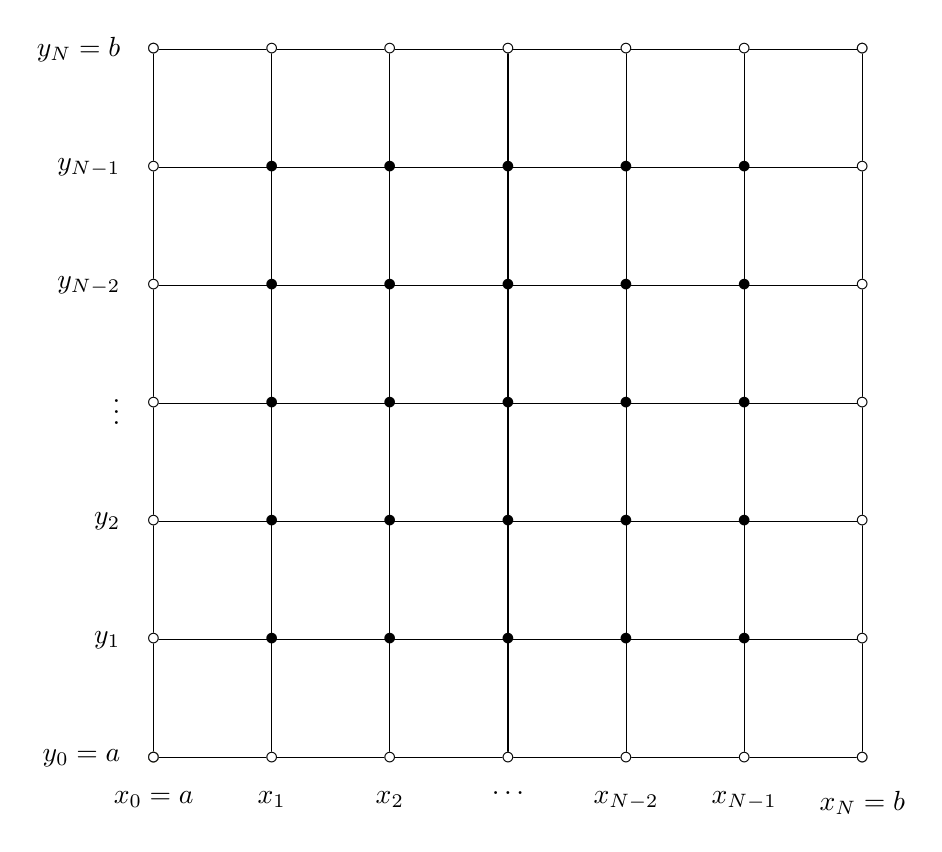
\begin{tikzpicture}[scale=1.5]
	\draw (-3,-3.2) node[below] {$x_0=a$} ;
	\draw (-2,-3.2) node[below] {$x_1$} ;
	\draw (-1,-3.2) node[below] {$x_2$} ;
	\draw (0,-3.2) node[below] {$\ldots$} ;
	\draw (1,-3.2) node[below] {$x_{N-2}$} ;
	\draw (2,-3.2) node[below] {$x_{N-1}$} ;
	\draw (3,-3.2) node[below] {$x_N =b$} ;
	
	\draw (-3.2,-3) node[left] {$y_0=a$} ;
	\draw (-3.2,-2) node[left] {$y_1$} ;
	\draw (-3.2,-1) node[left] {$y_2$} ;
	\draw (-3.2,0) node[left] {$\vdots$} ;
	\draw (-3.2,1) node[left] {$y_{N-2}$} ;
	\draw (-3.2,2) node[left] {$y_{N-1}$} ;
	\draw (-3.2,3) node[left] {$y_N =b$} ;
	
	\draw (-3,-3) grid[step=1] (3,3);

	\draw (-3,-3) node[color=yellow] {$\bullet$} ;
	\draw (-3,-3) node {$\circ$} ;
	
	\foreach \k in {-3,...,3}
		{\draw  (\k,-3) node[color=white] {$\bullet$} ;
	   	\draw (\k,-3) node {$\circ$} ;
	   	\draw  (\k,3) node[color=white] {$\bullet$} ;
	   	\draw (\k,3) node {$\circ$} ;
	   	\draw  (-3,\k) node[color=white] {$\bullet$} ;
	   	\draw (-3,\k) node {$\circ$} ;
	   	\draw  (3,\k) node[color=white] {$\bullet$} ;
	   	\draw (3,\k) node {$\circ$} ;
	   	}
	   	
	\foreach \k in {-2,...,2}
		{\draw  (\k,-2) node {$\bullet$};
		\draw  (\k,-1) node {$\bullet$};
		\draw  (\k,0) node {$\bullet$};
		\draw  (\k,1) node {$\bullet$};
		\draw  (\k,2) node {$\bullet$};
	   	}
\end{tikzpicture}
\end{center}
\caption{Grille en dimension 2. Les symboles $\circ$ désignent les points de bords, les symboles $\bullet$ désignent les points intérieurs de la grille.}
\label{fig:maillage2D}
\end{figure}

On dit qu'une fonction $u : (x,y) \in \mathbb{R} \mapsto u(x,y) \in \mathbb{R}$ est $L-$\textit{périodique} dans les directions $x$ et $y$ si 
\begin{equation}
\begin{array}{rcl}
u(x,y+L) & = & u(x,y) \\
u(x+L,y) & = & u(x,y)
\end{array} \text{ pour tous } (x,y) \in \mathbb{R}^2.
\end{equation}

Comme en dimension 1, nous définissons différentes notions de fonctions discrètes associées à la grille :
\begin{enumerate}
\item Une \textit{fonction de grille} est une fonction définie aux points de la grille $(x_i,y_j)_{0 \leq i,j \leq N}$. Nous notons ces fonctions en fonte gothique comme $\mathfrak{u}$ ou $\mathfrak{v}$. On a :
\begin{equation}
\mathfrak{u} = \left( \mathfrak{u}(x_i,y_j) \right)_{0 \leq i,j \leq N} \text{ et } \mathfrak{u}_{i,j} = \mathfrak{u}(x_i,y_j).
\end{equation}
$\mathfrak{u}$ est périodique si $\mathfrak{u}(x_{i},y_0) = \mathfrak{u}(x_{i},y_N)$ et $\mathfrak{u}(x_{0},y_j) = \mathfrak{u}(x_{N},y_j)$ pour tous $0 \leq i,j \leq N$.
On note $L^2_h$ l'espace des fonctions de grilles. Cet espace est équipé d'un produit scalaire et de la norme associée :
\begin{equation}
(\mathfrak{u}, \mathfrak{v})_h = h^2 \gsum_{i,j=0}^N \mathfrak{u}(x_i,y_j) \mathfrak{v}(x_i,y_j) \text{ et } |\mathfrak{u}|_h = \sqrt{(\mathfrak{u},\mathfrak{u})_h}.
\end{equation}
de plus, on a également
\begin{equation}
| \mathfrak{u} |_{\infty} = \max_{0 \leq i,j \leq N} |\mathfrak{u}(x_i,y_j)|.
\end{equation}
Pour simplifier les notations, nous noterons
\begin{equation}
\mathfrak{u}_{i,j} = \mathfrak{u}(x_i, y_j) \text{ avec } 1 \leq i,j \leq N.
\end{equation}

\item Soit $u : (x,y) \in \Omega \mapsto u(x,y) \in \mathbb{R}$, nous définissons la fonction associée, notée $u^*$ par la restriction de $u$ à la grille :
\begin{equation}
u^*_{i,j} = u(x_i, y_j) \text{ pour tous } 0 \leq i,j \leq N.
\end{equation}

Pour $u$ est périodique selon $x$ et $y$, on a $u^*_{i,0}=u^*_{i,N}$ et $u^*_{0,j}=u^*_{N,j}$ pour tous $0 \leq i,j \leq N$.
D'une manière générale, dans un contexte périodique, les données sur des bords opposés du carrés coïncident.

\item A une fonction de grille $\mathfrak{u}$, on associe un vecteur $U \in \mathbb{R}^{(N+1)^2}$ constitué des valeurs de $\mathfrak{u}$ dans l'ordre anti-lexicographique :
\begin{equation}
U = \begin{bmatrix}
\mathfrak{u}_{0,0}\\
\mathfrak{u}_{1,0}\\
\vdots \\
\mathfrak{u}_{N,0}\\
\mathfrak{u}_{0,1}\\
\mathfrak{u}_{1,1}\\
\vdots \\
\mathfrak{u}_{N,1}\\
\vdots \\
\mathfrak{u}_{N,N}\\
\end{bmatrix}.
\end{equation}
On note ces vecteurs par des lettres capitales. Les matrices de $\mathbb{M}_{(N+1)^2} (\mathbb{R})$, notée par des lettres latines capitales, agissent sur ces vecteurs.
\end{enumerate}

\begin{figure}[htbp]
\begin{center}
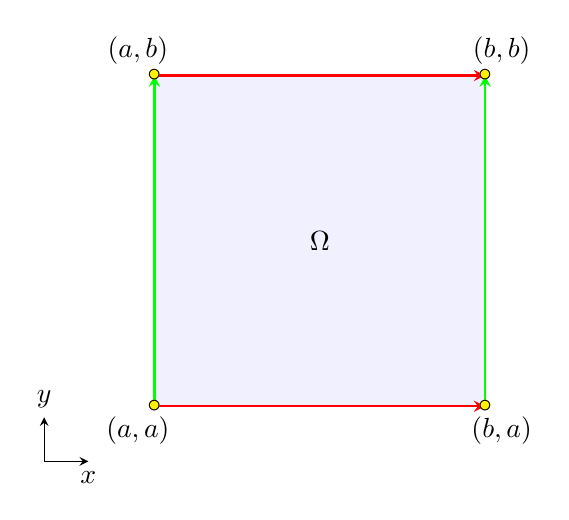
\begin{tikzpicture}[scale=.7]
	\filldraw[draw=black,fill=blue!30!white,opacity=0.20]
	plot (-3,-3) -- (-3,3)
	-- plot (-3,3) -- (3,3)
	-- plot (3,3) -- (3,-3)
	-- plot (3,-3) -- (-3,-3)
	-- cycle;

	\draw [>=stealth, ->,color=green,thick] (-3,-3) -- (-3,3) ;
	\draw [>=stealth, ->,color=green,thick] (3,-3) -- (3,3) ;
	\draw [>=stealth, ->,color=red,thick] (-3,-3) -- (3,-3) ;
	\draw [>=stealth, ->,color=red,thick] (-3,3) -- (3,3) ;
	
	\draw (-3.3,-3.45) node {$(a,a)$} ;
	\draw (3.3,-3.45) node {$(b,a)$} ;
	\draw (-3.3,3.45) node {$(a,b)$} ;
	\draw (3.3,3.45) node {$(b,b)$} ;
	\draw (0,0) node {$\Omega$} ;
	\draw  (-3,-3) node[color=yellow] {$\bullet$} ;
	\draw (-3,-3) node {$\circ$} ;
	\draw  (3,-3) node[color=yellow] {$\bullet$} ;
	\draw (3,-3) node {$\circ$} ;
	\draw  (-3,3) node[color=yellow] {$\bullet$} ;
	\draw (-3,3) node {$\circ$} ;
	\draw  (3,3) node[color=yellow] {$\bullet$} ;
	\draw (3,3) node {$\circ$} ;
	\draw [>=stealth, ->] (-5,-4) -- (-4.2,-4) ;
	\draw (-4.2,-4) node[below] {$x$} ;
	\draw [>=stealth, ->] (-5,-4) -- (-5,-3.2) ;
	\draw (-5,-3.2) node[above] {$y$} ;
\end{tikzpicture}
\end{center}
\caption{Carré périodique. Dans le contexte périodique, les données sur les bords de couleurs identiques coïncident. Les quatre coins du carré représentent la même donnée.}
\label{fig:period2D}
\end{figure}

















\subsection{Opérateurs en géométrie cartésienne}

En utilisant les notations de la partie \ref{sec:notation_2D} en contexte périodique, nous définissons des opérateurs agissant sur les fonctions de grilles en dimension 2.

\begin{definition}
Soient $\tau_x$ et $\tau_y$ les \textit{opérateurs de translation} dans les directions $x$ et $y$ définis par
\begin{equation}
\left\lbrace
\begin{array}{rcl}
\tau_x \mathfrak{u}_{i,j} & = & \mathfrak{u}_{i+1,j}\\
\tau_y \mathfrak{u}_{i,j} & = & \mathfrak{u}_{i,j+1}\\
\end{array}
\right.
\end{equation}
avec $\mathfrak{u}$ une fonction de grille et $1 \leq i,j \leq N$.
\end{definition}

Les opérateurs obtenus en dimension 1 sont définis en dimension 2 grâce à ces deux opérateurs de translation. On définit les opérateurs centrés dans les directions $x$ et $y$ par 
\begin{equation}
\left\lbrace
\begin{array}{rcl}
\delta_x & = & \dfrac{\tau_x - \tau_x^{-1}}{2h} \\
\delta_y & = & \dfrac{\tau_y - \tau_y^{-1}}{2h}
\end{array}
\right.
\label{eq:der_centrée_2D}
\end{equation}
De la même manière, on définis les opérateurs de Simpson dans chaque direction par 
\begin{equation}
\left\lbrace
\begin{array}{rcl}
\sigma_x & = & \dfrac{1}{6} \tau_x + \dfrac{4}{6} id + \dfrac{1}{6} \tau_x^{-1} \\
\sigma_y & = & \dfrac{1}{6} \tau_y + \dfrac{4}{6} id + \dfrac{1}{6} \tau_y^{-1} \\
\end{array}
\right.
\label{eq:simpson_2D}
\end{equation}
Chacun des opérateurs $\sigma_x$ et $\sigma_y$ est inversible.
L'opérateur hermitien en dimension 1 $\delta_x^H$ est étendue en dimension 2 grâce à la relation suivante 
\begin{equation}
\left\lbrace
\begin{array}{rcl}
\delta_x^H & = & \sigma_x^{-1} \circ \delta_x \\
\delta_y^H & = & \sigma_y^{-1} \circ \delta_y
\end{array}
\right.
\label{eq:der_herm_2D}
\end{equation}

\begin{theoreme}
Soit $u : x \in \Omega \mapsto u(x) \in \mathbb{R}$ est une fonction de $\mathcal{C}^5 (\Omega)$. On note $u^*$ la fonction de grille associée à $u$ et $u_x^*$ (resp. $u_y^*$) la fonction de grille associée à la dérivée de $u$ dans la direction $x$ (resp. $y$) notée $\partial_x u$ (resp. $\partial_y u$). Alors
\begin{equation}
\begin{array}{rcl}
|u^*_{x} - \delta_x^H u^*|_{\infty} &\leq& C h^4\\
|u^*_{y} - \delta_y^H u^*|_{\infty} &\leq& C h^4
\end{array}
\end{equation}
\end{theoreme}

\begin{proof}
Conséquence du théorème \ref{prop:consistence_herm2} appliqué dans chaque direction $x$ et $y$.
\end{proof}













\subsection{Ecriture matricielle des opérateurs en dimension 2}

Dans cette section, nous précisons les notations vectorielles et matricielles utiles à l'écriture matricielle des opérateurs en dimension 2.

Nous définissons la \textit{base canonique} de $\mathbb{R}^N$, notée $\left(e_i \right)_{1 \leq i \leq N}$ et donnée par 
\begin{equation}
\left( e_i \right) = \delta_{i,j} = \left\lbrace
\begin{array}{rl}
1 & \text{ si } j=i,\\
0 & \text{ sinon.}
\end{array}
\right.
\end{equation}
$\delta_{i,j}$ est le symbole de Kronecker.

\begin{definition}
Soit $A$ une matrice de taille $m \times n$ et $B$ une matrice de $p \times q$, avec $m, n, p, q \in \mathbb{N}^{\star}$. La matrice $A \otimes B$ est une matrice de taille $mp \times nq$ donnée comme le produit de Kronecker de $A$ par $B$ et 
\begin{equation}
A \otimes B = 
\begin{bmatrix}
a_{1,1}B & \cdots & a_{1,n}B \\ 
\vdots & \ddots & \vdots \\ 
a_{n,1}B & \cdots & a_{n,n}B
\end{bmatrix} 
\end{equation}
\end{definition}
On rapelle les propriétés suivantes concernant le produit de Kronecker :

\begin{proposition}
Soient $A$, $B$, $C$ et $D$ des matrices et $\alpha$ un réel.
\begin{itemize}
\item La multiplication par un scalaire vérifie
\begin{equation}
\alpha ( A \otimes B ) = \alpha A \otimes B = A \otimes \alpha B,
\end{equation}

\item si les produits $AC$ et $BD$ sont bien définis alors
\begin{equation}
(A \otimes B ) (C \otimes D) = AC \otimes BD,
\end{equation} 


\item si $A$ et $B$ sont inversibles
\begin{equation}
(A \otimes B)^{-1} = A^{-1} \otimes B^{-1}.
\end{equation}
\end{itemize}
\label{prop:pdt_kron}
\end{proposition}
L'application $\text{vec}_2$ permet de transformer une fonction de grille $\mathbf{u}$ en un vecteur $U$.

\begin{definition}
L'opérateur $\text{vec}_2$ est défini par
\begin{equation}
\begin{array}{rcl}
\text{vec}_2 : L^2_h & \longrightarrow & \mathbb{R}^{N^2}\\
\mathfrak{v} & \longrightarrow & V = \text{vec}_2(\mathfrak{v})
\end{array}
\end{equation}
avec
\begin{equation}
\text{vec}_2(\mathfrak{v}) = \gsum_{i,j=1}^N \left( e_j \otimes e_i \right)\mathfrak{v}_{i,j}.
\end{equation}
\end{definition}

L'opérateur $\text{vec}_2$ transforme une fonction de grille $\mathfrak{v}$ en un vecteur en organisant les données dans l'ordre antilexicographique. Si $V = \text{vec}_2 (\mathfrak{v})$ alors on a l'égalité suivante :
\begin{equation}
V=[\mathfrak{v}_{1,1}, \mathfrak{v}_{2,1}, \mathfrak{v}_{3,1}, \cdots, \mathfrak{v}_{N,1}, \mathfrak{v}_{1,2}, \mathfrak{v}_{2,2}, \cdots,  \mathfrak{v}_{N-1,N}, \mathfrak{v}_{N,N}]^T
\end{equation}

\begin{proposition}
Soit $\mathfrak{u}$ une fonction de grille. Alors les opérateurs de dérivées centrées \eqref{eq:der_centrée_2D} s'écrivent matriciellement sous la forme
\begin{equation}
\left\lbrace
\begin{array}{rcl}
\text{vec}_2(\delta_x \mathfrak{u}) & = & (Id \otimes K) \text{vec}_2(\mathfrak{u})\\
\text{vec}_2(\delta_y \mathfrak{u}) & = & (K \otimes Id) \text{vec}_2(\mathfrak{u})\\
\text{vec}_2(\sigma_x \mathfrak{u}) & = & (Id \otimes P) \text{vec}_2(\mathfrak{u})\\
\text{vec}_2(\sigma_y \mathfrak{u}) & = & (P \otimes Id) \text{vec}_2(\mathfrak{u})\\
\end{array}\right.
\end{equation}
\label{prop:op_der_simpson_mat}
\end{proposition}

\begin{proof}
Par définition de $\text{vec}_2$, on a 
\begin{align*}
\text{vec}_2 (\delta_x \mathfrak{u}) &=& \gsum_{i,j=1}^N (e_j \otimes e_i) \delta_x \mathfrak{u_{i,j}} \\
	&= \dfrac{1}{2h} \gsum_{i,j=1}^N (e_j \otimes e_i) \left( \mathfrak{u}_{i+1,j} - \mathfrak{u}_{i-1,j} \right) \\
	&= \dfrac{1}{2h} \gsum_{i,j=1}^N e_j \otimes e_i \mathfrak{u}_{i+1,j} - e_j \otimes e_i \mathfrak{u}_{i-1,j}\\
	&= \dfrac{1}{2h} \gsum_{i,j=1}^N e_j \otimes (e_i \mathfrak{u}_{i+1,j}-e_i \mathfrak{u}_{i-1,j}) \\
	&= (Id \otimes K) \text{vec}_2(\mathfrak{u}).
\end{align*}
les autres égalités se montrent de la même manière
\end{proof}

De ces égalités, il découle le calcul matriciel de $\delta_x^H \mathfrak{u}$ et de $\delta_y^H \mathfrak{u}$.

\begin{theoreme}
Soit $\mathfrak{u}$ une fonction de grille. Alors, si on pose 
\begin{equation}
\left\lbrace
\begin{array}{rcl}
U & = & \text{vec}_2 (\mathfrak{u}) \\
U_x & = & \text{vec}_2 (\delta_x^H \mathfrak{u}) \\
U_y & = & \text{vec}_2 (\delta_y^H \mathfrak{u}) \\
\end{array}
\right.
\end{equation}
alors les égalités suivantes sont vérifiées
\begin{equation}
\left\lbrace
\begin{array}{rcccl}
U_x &=& (Id \otimes P)^{-1}(Id \otimes K) U &=& (Id \otimes P^{-1}K)U \\
U_y &=& (P \otimes Id)^{-1}(K \otimes Id) U &=& (P^{-1}K \otimes Id)U\\
\end{array}
\right.
\end{equation}
\end{theoreme}

\begin{proof}
Conséquence directe des propositions \ref{prop:op_der_simpson_mat} et \ref{prop:pdt_kron}.
\end{proof}

La matrice du schéma hermitien $(Id \otimes P^{-1}K)$ en direction $x$ et $(P^{-1}K \otimes Id)$ en direction $y$ vérifient des propriétés d'antisymétriques similaires à celles en dimension 1.
\begin{proposition}
Les matrices $(Id \otimes P^{-1}K)$ et $(P^{-1}K \otimes Id)$ sont antisymétrique.
\end{proposition}

\begin{proof}
$P^{-1}K$ est antisymétrique. D'où le résultat.
\end{proof}















